\section{跨层性能观测工具链选型}\label{sec:tool-selection}

在线推理循环本身只有几十毫秒的时间尺度，因此测量工具不能明显改变被测对象的运行节奏。
本节先比较 strace 和 ftrace 两类常用工具，再用同一条推理循环实测它们带来的扰动，
最后确定后续章节采用的内核态追踪方案。
这种先校准测量工具、再解释系统瓶颈的做法，也符合系统性能分析中强调的
“先确认观测开销，再分析被测系统”的基本原则。

strace\cite{strace} 的优点是使用方便，能够直接看到进程发起了哪些系统调用。
但它的工作方式决定了开销较大：目标进程每进入或退出一次系统调用，
都会被 ptrace 暂停，并切换到 strace 进程读取参数和返回值。
在摄像头读取、串口通信和线程同步都很频繁的在线推理循环中，
这种逐次拦截会放大上下文切换次数，进而改变原本的帧率和阶段耗时结构。
因此，strace 更适合用来定性确认调用类型，而不适合作为正式的定量时序依据。

ftrace\cite{ftrace} 的记录位置更靠近内核。
系统调用、调度或自定义事件触发后，内核直接把记录写入内部缓冲区，
不需要为每一次事件切换到单独的跟踪进程，所以插桩本身对主循环的干扰更小。
对本文而言，ftrace 的另一个关键优点是可以把标准内核事件和自定义内核日志放在同一条追踪流中。
例如，系统调用事件负责记录 sys\_pselect6、sys\_futex 的进入和退出，
自编译内核中的 trace\_printk 则负责输出 do\_select 和
do\_futex 内部的总耗时、睡眠时间和 CPU 时间等细分信息。
这些记录最终共享同一个 ftrace 缓冲区、同一套时间戳、CPU 编号和进程信息，
因此可以直接把 Python 主循环、摄像头等待和 futex 线程同步放到同一条时间线上分析，
不需要再在用户态日志和内核日志之间额外做时钟校准。
不过，ftrace 也不是完全无代价：采集结束后导出 trace 文件，
或在采集过程中持续读取 trace\_pipe，都会产生额外的文件读写、CPU 占用和内存带宽消耗；
当事件过于密集时，缓冲区还可能覆盖旧记录。
因此，本文不仅比较 strace 和 ftrace，
也进一步区分 ftrace 的延迟导出和实时导出两种使用方式。

为定量比较这些工具对主循环的影响，本文设计了测量工具校准实验。
实验固定 chunk\_size 为 100、目标帧率为 30\,fps，并在约 30\,s 的同一类推理循环上比较四组配置。
A 组为基准组，不开启任何追踪；B 组使用 strace -f -ttT 包裹运行命令；
C 组只让 ftrace 写入内核缓冲区，待单段数据采集结束后再导出文件；
D 组同样开启 ftrace，但同时启动后台进程持续读取 trace\_pipe 并写入文件。
帧率、上下文切换次数和阶段时间占比由在线控制程序通过
resource.getrusage 与 sysfs 自动采集，并写入
analysis/timing\_stats.csv。表~\ref{tab:tool-overhead} 汇总了四组的核心结果。

\begin{table}[htbp]
  \centering
  \caption{四组测量工具对主循环的扰动（每组 $n=1$，仅用于工具选型）}
  \label{tab:tool-overhead}
  \begin{tabular}{lcccc}
    \toprule
    指标 & A 基准 & B strace & C ftrace 延迟 & D ftrace 实时 \\
    \midrule
    平均帧率              & 16.13   & 9.53    & 13.89  & 12.48  \\
    相对 A 的帧率下降               & ---     & $-40.9\%$ & $-13.9\%$ & $-22.6\%$ \\
    系统态耗时        & 1.40    & 2.76    & 1.37   & 1.03   \\
    自愿上下文切换          & 23{,}947  & 750{,}662 & 30{,}377 & 36{,}336 \\
    非自愿上下文切换        & 78{,}436  & 541{,}334 & 84{,}481 & 52{,}907 \\
    观测占比漂移     & 0       & $+34.8$ pp & $-5.5$ pp & $-3.0$ pp \\
    等待占比漂移    & 0       & $-31.6$ pp & $-0.9$ pp & $-0.8$ pp \\
    追踪文件大小                   & ---     & 157\,MB & 168\,MB & 823\,MB \\
    \bottomrule
  \end{tabular}
\end{table}

从平均帧率看，strace 对主循环的影响最明显。
如图~\ref{fig:tool-fps} 所示，B 组的平均帧率从 A 组的 16.13\,fps 降至 9.53\,fps，
下降幅度达到 40.9\%。这一变化已经足以说明，
在当前负载下用 strace 采集到的时序数据不能代表真实运行状态。
C 组和 D 组同样会降低帧率，但下降幅度分别为 13.9\% 和 22.6\%，
明显小于 B 组。虽然单次校准实验还不能给出严格的统计方差，
但三组之间的相对关系非常清楚：延迟导出的 ftrace 扰动最小，
实时导出的 ftrace 次之，strace 最大。

\begin{figure}[H]
  \centering
  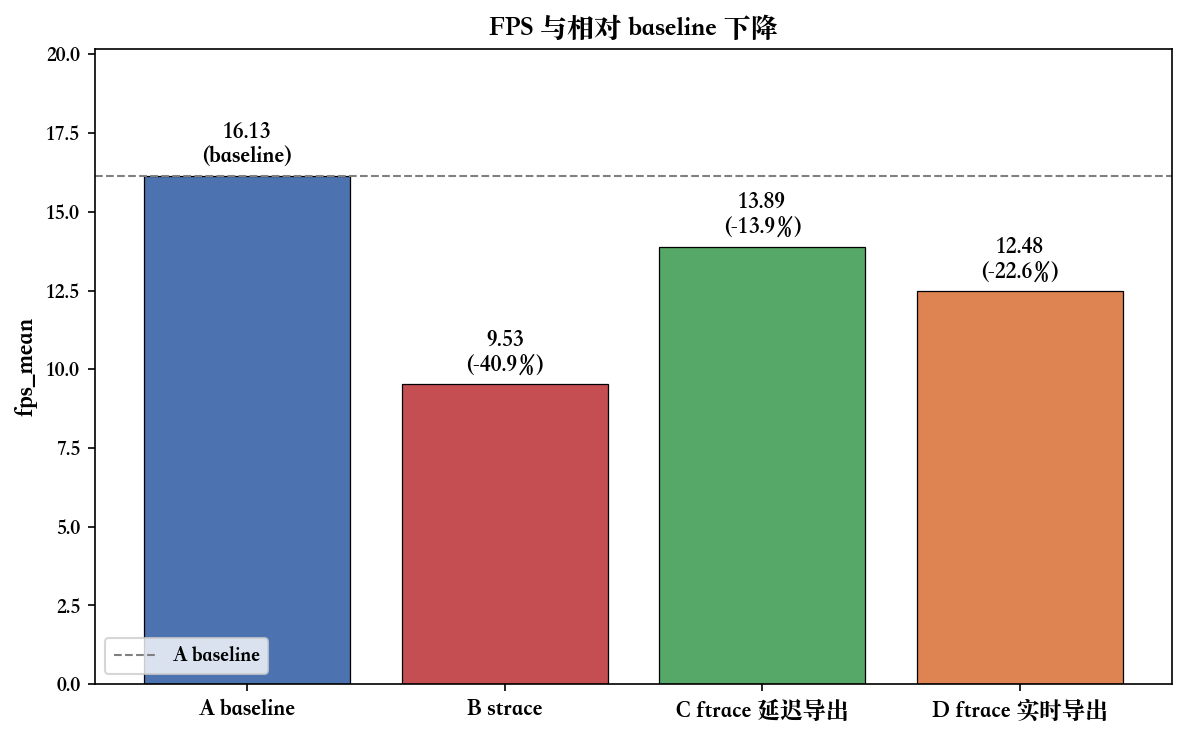
\includegraphics[width=0.85\textwidth]{实验/04_实验环境与测量工具校准/fps_drop.png}
  \caption{四组测量工具下的平均帧率与相对 A 组的下降百分比}
  \label{fig:tool-fps}
\end{figure}

上下文切换次数进一步解释了帧率下降的来源。
图~\ref{fig:tool-cs} 使用对数坐标展示四组的自愿和非自愿上下文切换次数。
B 组的自愿上下文切换从 A 组的约 2.4 万次增加到约 75 万次，
非自愿上下文切换也从约 7.8 万次增加到约 54 万次。
这里需要区分“工具引起的帧率下降”和“系统原有瓶颈”。
A 组的 16.13\,fps 反映了树莓派5 在当前 ACT 策略、双相机输入和舵机通信配置下的原始运行能力；
B、C、D 三组并不用于评价机器人控制程序本身，而是用于衡量测量工具是否改变了这个基准。
因此，工具选型时更关注相对 A 组的下降幅度，而不是某一组是否达到 30\,fps 的目标值。
B 组下降超过 40\%，说明 strace 已经把被测系统推入了另一个运行状态：
观测阶段中的系统调用不再只是等待设备事件，而会被调试器反复截获、唤醒和恢复。
相比之下，C 组只把事件写入内核缓冲区，采集过程中没有持续的用户态读取进程参与；
D 组虽然额外读取 trace\_pipe，但其扰动仍显著低于 strace。
这也是本文将 ftrace 延迟导出作为正式实验默认方案的直接依据。

这种数量级上的放大正是 ptrace 机制的直接结果：
摄像头链路中密集出现的 pselect6、read、ioctl 等系统调用，
都会被 strace 反复打断和恢复。
相比之下，C 组的上下文切换次数只比 A 组略高，
D 组的额外切换主要来自后台读取 trace\_pipe 的进程。
这说明 ftrace 写入内核缓冲区这一步本身并不会显著扰动调度路径。

\begin{figure}[H]
  \centering
  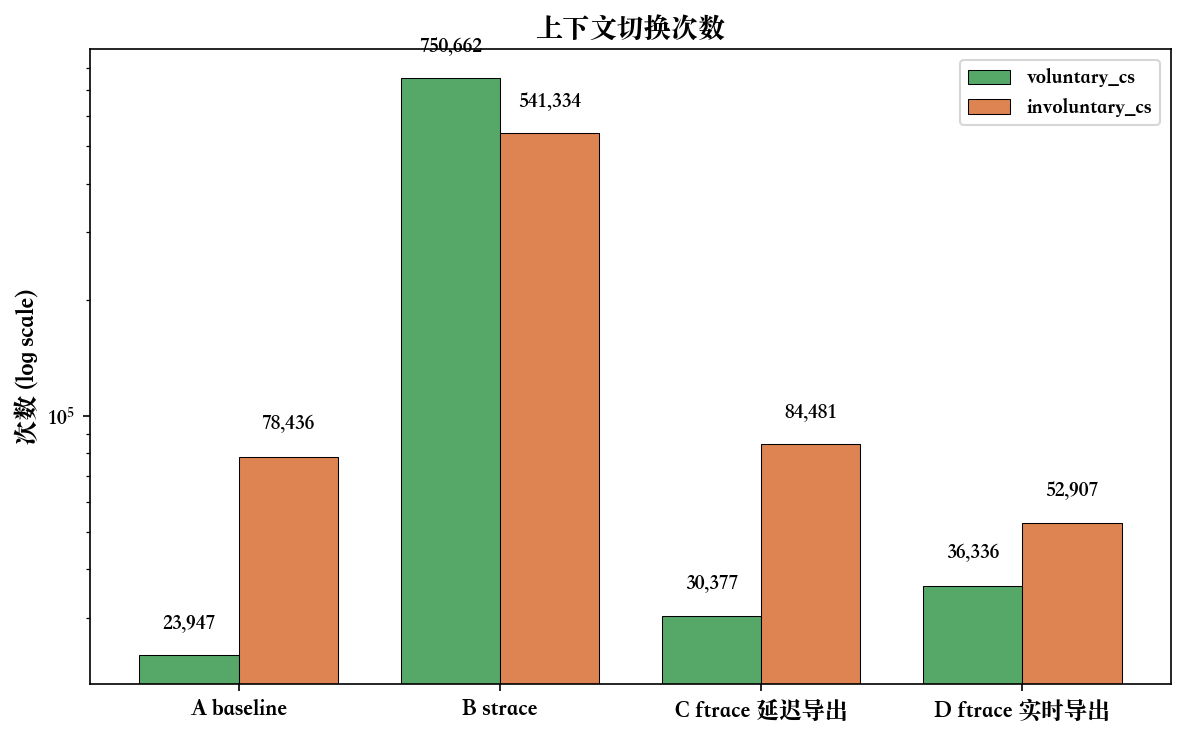
\includegraphics[width=0.85\textwidth]{实验/04_实验环境与测量工具校准/context_switches.png}
  \caption{四组的自愿与非自愿上下文切换次数（对数坐标）}
  \label{fig:tool-cs}
\end{figure}

阶段占比的变化说明，工具扰动不仅会影响总帧率，也会改变各阶段之间的相对关系。
图~\ref{fig:tool-phase} 中的数值表示相对 A 组的百分点偏移。
图中的灰色虚线表示设计阶段提出的 $\pm 3$ 个百分点验收阈值。
B 组的观测阶段占比增加 34.8 个百分点，等待阶段占比减少 31.6 个百分点，
说明 strace 把摄像头读取等系统调用密集的部分严重拉长，
并挤压了原本用于补足帧间隔的等待阶段。
从上下文切换类型看，自愿上下文切换通常对应线程主动进入阻塞等待，
例如等待摄像头帧就绪、等待串口返回或等待 futex 唤醒；
非自愿上下文切换则更多来自调度器抢占、时间片耗尽或被更高优先级任务打断。
strace 会同时放大这两类切换：
目标进程进入系统调用时先被内核暂停并通知 strace，
strace 读取系统调用号、参数和返回值后再恢复目标进程，
系统调用退出时还会重复一次类似过程。
因此，在摄像头、串口和线程同步事件本来就高频出现的在线推理循环中，
ptrace 带来的额外调度开销会迅速累积为数量级差异。
ftrace 的缓冲区写入发生在内核路径内部，不需要每个事件都切回用户态分析进程，
所以 C 组的上下文切换规模更接近 A 组。

这种结构性扭曲比单纯的帧率下降更严重，
因为它会让后续瓶颈分析把工具带来的开销误判为程序自身的观测开销。
C 组和 D 组虽然也有漂移，但幅度明显较小，
等待阶段和动作写入阶段的变化都不超过 1 个百分点，
没有出现 B 组那样的阶段结构重排。

\begin{figure}[H]
  \centering
  
\includegraphics[width=0.98\textwidth]{实验/04_实验环境与测量工具校准/phase_drift.png}
  \caption{阶段占比漂移}
  \label{fig:tool-phase}
\end{figure}

综合帧率、上下文切换和阶段占比三方面结果，本文在正式实验中采用
ftrace 延迟导出作为主要内核态时序采集方式。
该方案的上下文切换次数和阶段时间结构最接近 A 组，
是本次校准中对单段推理循环扰动最小的方案。
当单段数据时长增加、内核缓冲区接近溢出时，
再使用实时导出作为后备方案。本文的缓冲区配置为每个 CPU 32\,MB，
树莓派5 四个核心合计 128\,MB；实时导出的代价是追踪文件从 168\,MB 增至 823\,MB，
约为延迟导出的 4.9 倍，但在存储空间上仍然可以接受。
strace 不参与最终定量分析，只在早期用于确认系统调用类型分布。

标准 ftrace 事件只能告诉本文某个系统调用何时进入、何时退出以及返回值是什么，
但无法继续拆分系统调用内部到底是在睡眠等待，还是在 CPU 上处理数据。
为了获得更细的时间分解，本文在自编译内核中加入了少量源码级插桩：
通过 trace\_printk 将自定义计时信息写入同一个 ftrace 缓冲区，
再与标准事件一起导出分析。

第一处插桩位于 pselect6 的内核实现路径，
具体位置是 fs/select.c 中的 do\_select 函数。
该函数是摄像头等待帧就绪时的重要入口。
本文在函数入口记录起始时间，在 poll\_schedule\_timeout 前后记录阻塞睡眠时间，
并在函数退出时输出总耗时、睡眠时间、上下文处理时间、返回值、就绪文件描述符以及设备路径。
这样一来，追踪结果中可以直接区分
“fd=8, file=video0” 对应的手眼摄像头和
“fd=9, file=video2” 对应的固定摄像头。
实测中，每次摄像头等待约为 30\,ms，其中睡眠时间约占总耗时的 99.7\%，
说明该路径主要是在等待新帧，而不是在 CPU 上持续计算。

第二处插桩位于 kernel/futex/syscalls.c 中的 do\_futex 函数。
该路径与 Python 运行时和 PyTorch 线程同步有关。
本文在函数入口以及 futex\_wait\_multiple 前后打点，
输出操作码、返回值、总耗时、CPU 时间和睡眠时间。
有了这组信息，就可以区分快速唤醒和长时间等待：
实测中，WAKE 操作的耗时通常在微秒级，
而 WAIT 操作的睡眠时间最高可达 1.8\,s。
这为后续判断 Python 线程间是否存在明显锁等待提供了依据。

这些自定义信息难以通过标准 tracepoint 或 kprobe 动态插桩稳定获得。
标准 tracepoint 不提供系统调用内部的时间拆分；
而在 kprobe 回调中解析文件描述符路径存在死锁风险。
相比之下，在 do\_select 的原生执行上下文中调用 d\_path 更可控。
因此，本文选择承担自编译内核的成本，换取更可靠的内核内部时间分解。
